\section{Direct reconstruction protocol and reproducibility}
\label{app:direct-protocol}

The protocol in \path{extensions/direct_reconstruction/PROTOCOL.md}
specifies the model, input preparation, optimization, analysis, and
exact task roster. Its public checkpoint includes the implementation,
numerical dependencies, source metadata, and prepared input arrays and
precedes evaluation on D. The exploratory gate-training pilot has a
separate design and does not contribute observations to the primary
interval family.

\paragraph{Local shape controls and gate normalization.}
Use the row-stored reference matrix, principal basis, and center from
Section~\ref{sec:direct-reconstruction}. Let $b(c)$ be the partition
block containing local model $c$, and set
\[
 a_c(z)=\mu_c+P_cP_c^\top(z-\mu_c),\quad
 u_c(z)=P_c^\top(z-\mu_c),\quad
 n_c(z)=(I_L-P_cP_c^\top)(z-\mu_c).
\]
The scalars $t_c$ and $e_c$ are the positive reference-radius and
projection-residual scales in Equation~\eqref{eq:nf-locality-gates}.
For a horizon-specific shape parameter $\xi_b$, the affine control uses
\[
 r_c^{\mathrm A}(z;\xi_b)=\mu_c+e^{\xi_b}P_cP_c^\top(z-\mu_c).
\]
Both this reconstruction and the KAHM reconstruction determine a folding
score $s_c$ through Equation~\eqref{eq:nf-folding-gates}. Their gate
logit is
$\ell_c(z)=16\log[1-\operatorname{clip}_{[0,1]}s_c(z)+10^{-6}]$.
The other two controls use logits
\begin{align*}
 \ell_c^{\mathrm{loc}}(z;\xi_b)
 &=-e^{\xi_b}\frac{\|n_c(z)\|_2^2}{e_c}
   -0.1e^{-\xi_b}\frac{\|z-\mu_c\|_2^2}{t_c},\\
 \ell_c^{\mathrm{RBF}}(z;\xi_b)
 &=-\frac{e^{\xi_b}\|u_c(z)\|_2^2+
                e^{-\xi_b}\|n_c(z)\|_2^2}{2t_c}.
\end{align*}
For every family, the temperature parameter $\eta_b$ gives the gate
\[
 \phi_c(z)=\frac{\exp\{e^{\eta_b}\ell_c(z)\}}
 {\sum_{j\in\mathcal C_b}\exp\{e^{\eta_b}\ell_j(z)\}},
 \qquad c\in\mathcal C_b.
\]
Both parameters lie in $[-\log4,\log4]$. The fixed model sets both to
zero, the gate-trained model fixes $\xi_b=0$, and the shape-trained
model fits both. The principal coordinates $u_c$ themselves remain
fixed in all three procedures.

The optimizer is L-BFGS-B with numerical forward differences, at most
40 iterations, at most 20 line-search steps per iteration, function
tolerance $10^{-10}$, and gradient tolerance $10^{-6}$. Its 256-evaluation
ceiling counts actual objective calls, including calls used for numerical
differentiation. A zero parameter vector initializes every optimization,
and the best finite evaluated parameter vector supplies the fitted state.

\paragraph{Exploratory gate-training pilot.}
The pilot used three independent seeds per law, separately implemented
generators, and at most 160 objective evaluations. Gate-temperature
training reduced mean KAHM MSE relative to its fixed version by 0.53\%
on nonlinear AR, 30.21\% on Van der Pol, and 11.29\% on Duffing. The
best directly trained local control was more accurate on every law;
raw RBF was also substantially stronger on Van der Pol and Duffing.
The reproduction materials contain all 99 method--task prediction
records and their optimization outcomes. These nine exploratory tasks
are excluded from the direct-reconstruction interval family.

\paragraph{Chronology and seasonal prediction.}
Synthetic seeds are 84200--84211 for each law, with
72-observation episodes and thirteen forecast origins per episode.
Implementation checks use seed 932001, outside the evaluation roster.
Whole-episode inner validation selects the raw baseline in A. For natural
data, inner A training targets must have matured by its first
validation query. Every outer target lies inside its segment. A history
can include observations from the preceding segment because these have
already been observed at the forecast origin. No future missing-value
imputation or label-based series replacement is used.

Dominick has history 52, offsets $(1,2,4)$ and seasonal period 52.
Rideshare uses only \texttt{price\_mean} series, history 24, offsets
$(1,3,6)$ and period 24. An A-only availability check reduced the
proposed history from 48 to 24 before the public checkpoint and any
forecast evaluation; the seasonal period and eligibility threshold
were unchanged. Wikipedia has history 28, offsets $(1,3,7)$ and
period 7. Sunspot uses the last 4,096 observations independent of their
values, history 28, offsets $(1,3,7)$ and period one. Each of the first
three collections contributes three hash-selected eligible series;
sunspot contributes its single series. Every source record, archive
checksum, selected identifier, original origin index, split boundary and
training-only scale is included in the reproduction records. Natural row caps are 512/128/128/128.
The minimum A eligibility is 96 complete windows with a positive finite
scale. A later unavailable segment remains a recorded failure. The three selected
rideshare series have no complete B windows, identified during preparation
after A-only selection; all three are retained as planned feasibility
failures. This precludes a complete four-collection accuracy aggregate.

Synthetic task MSE averages squared errors over the three offsets and
all D origins. Natural task MSE is divided by an A-only scale: the mean
of finite squared differences at the collection's seasonal period. If
this mean is unavailable, nonfinite, or nonpositive, the corresponding
first-difference mean is used. A task with no positive finite scale is
ineligible. The scale remains fixed throughout selection and evaluation.
All source-level means weight the selected series equally.

For a primary synthetic comparison, let $d_r$ be comparator MSE minus
reconstruction-trained KAHM MSE in repetition $r$, for $r=1,\ldots,12$.
With sample mean $\bar d$ and sample standard deviation $s_d$, the
95\% Bonferroni-adjusted interval is
\[
 \bar d\ \pm\ t_{11,1-0.05/(2\cdot18)}\frac{s_d}{\sqrt{12}},
\]
where $t_{\nu,q}$ denotes the $q$ quantile of Student's $t$ distribution
with $\nu$ degrees of freedom. Under independent normal paired
differences, these intervals jointly cover all eighteen population mean
differences with probability at least 95\%; otherwise the coverage
uses a normal approximation. The statistical unit is the complete
repetition, not an individual forecast origin.

Seasonal naive predicts each offset from the most recent observed value
with the appropriate seasonal phase. For period $p$ this is
$y_{t+h-p\lceil h/p\rceil}$, using only indices at or before $t$.
Period one therefore gives persistence. All declared histories include
the required seasonal lag. The selected source records are
\url{https://doi.org/10.5281/zenodo.4654802},
\url{https://doi.org/10.5281/zenodo.5122114},
\url{https://doi.org/10.5281/zenodo.4656080}, and
\url{https://doi.org/10.5281/zenodo.4654773}; the source manifest retains
attribution and archive-license metadata.

\paragraph{Baseline and correction selection.}
Raw RBF and boosting retain the fitted ridge state for a recorded
horizon-wise D fallback; a D failure cannot change their C forecast or
the C-selected policy. Its baseline cost and serialized bytes are included.
Raw ridge uses penalties $10^{-4},10^{-3},10^{-2},10^{-1},1,10,100$,
selected inside A and then refitted on A. The raw RBF reference retains
raw standardized history together with at most 64 Nystr\"om landmarks;
bandwidth factors $0.5,1,2$ multiply the median positive landmark
squared-distance scale, and B selects among them and the same seven
penalties.
Histogram gradient boosting fits 100 iterations with L2 penalty one,
learning rate $0.05$ or $0.1$, and maximum leaves 7 or 15; B selects the
grid jointly across horizons without external early stopping, using
a separate fitted tree ensemble per target. All local corrections use the
same A residual targets, sum-loss penalties $0.01,0.1,1$, A-standardized
features and unpenalized intercept. C chooses their mixing weights
separately by horizon with the zero-correction tie-breaking rule. A budget exit or
nonfinite trial is logged; the best finite incumbent is retained.

The affine gain and locality/RBF anisotropy are deliberately different
functional interventions from the KAHM bandwidth. Their common parameter
counts, supervision and evaluation ceilings support a matched experiment
at that level; they do not prove equal approximation power or equal
computation. Likewise, a gate-only arm has three parameters per horizon
and a reconstruction/shape arm has six, so their comparison asks whether
the additional intervention helps within the declared budget.

\paragraph{Computation and state.}
Numerical-library thread counts are fixed to one. Warm measured nodes
cover the baseline, shared bank, KAHM-specific factors, all paid geometry
trials, C selection, and D transformations and predictions. The implementation eagerly prepares
fixed gate queries and charges that work even when C selects zero
correction or a different bandwidth; the accounting is conservative
relative to a possible lazy implementation.
Each standalone procedure sums its required dependencies once. Policy
costs sum the union of measured candidate dependencies, including their
eager query work, not only the selected winner. This component sum is not
a separately timed minimal policy execution. Selected fitted states, their serialized byte sizes and
serialization time are retained. Downloads, input preparation, imports
and evidence artifact writing lie outside the model pipeline. Absolute
times and ratios describe this implementation and host, not intrinsic
algorithmic constants. A whole-process high-water RSS is not a
per-method memory estimate.

The evaluation compares fixed computational search budgets rather than
equal measured wall times. It does not evaluate delayed-label updates
or drifting streams; those questions are addressed separately in
Section~\ref{sec:adaptive-development}.

\paragraph{Computational verification.}
The verification program checks archived inputs and source files, reconstructs
windows from retained raw episodes or series, recomputes C/D losses,
checks all method and candidate rosters, replays strict selection,
checks exact zero correction, reconstructs cost dependencies and
replays serialized selected predictions. The program passes 543,017 consistency checks, including reconstruction
of 144 generated episode batches and replay of 731 selected states on
C and D. A separate calculation recomputes scalar losses, A-only
natural scales, and all 18 intervals without importing the model or
its analyzer. Neither check independently refits every optimization
trial or supplies an external experimental replication.

Bitwise regeneration also depends on the numerical environment. The
recorded execution uses NumPy 2.3.5 on an AVX512-capable x86-64 host.
A post-execution diagnostic reproduces all four episode batches of one
declared Duffing task exactly on that host, but disabling AVX512 dispatch
changes some values at floating-point roundoff scale. Package versions
and single-thread execution alone therefore do not guarantee identical
regenerated bytes on other processors. The archived input arrays therefore provide the exact evaluated inputs.
Regeneration checks compare their bytes exactly, whereas selected-state
prediction replay uses an absolute and relative tolerance of $10^{-10}$.
A separate raw-RBF state probe crosses the declared $10^{-10}$ absolute
and relative replay tolerances under altered dispatch, while changing
its C/D mean squared errors by less than $10^{-14}$ relatively.
Verification succeeds on the original host and on one compatible hosted
environment. The altered-dispatch failures identify a limitation of
strict numerical replay across processor configurations.


\subsection{Complete comparisons and resource records}

\begin{table}[!htbp]
\centering\small
\setlength{\tabcolsep}{4pt}
\caption{The complete 18-comparison family for reconstruction-trained
KAHM. With $\overline L$ denoting mean MSE across twelve repetitions,
gain is $100(\overline L_{\rm control}-\overline L_{\rm KAHM})/
\overline L_{\rm control}$. Intervals are absolute paired MSE differences,
not percentage intervals; their positive direction favors KAHM.}
\label{tab:direct-primary}
\begin{tabular}{llrrl}
\toprule
Law & Control & Gain (\%) & Difference interval & Outcome \\
\midrule
AR & Raw RBF & 2.87 & [6.65e-06, 0.000278] & positive \\
AR & Gate KAHM & 0.09 & [-3.86e-05, 4.71e-05] & unresolved \\
AR & Reconstruction affine & -0.11 & [-0.0001, 8.97e-05] & unresolved \\
AR & Reconstruction locality & 1.11 & [-3.46e-05, 0.000142] & unresolved \\
AR & Reconstruction RBF-local & -0.18 & [-9.5e-05, 7.77e-05] & unresolved \\
AR & Selected non-KAHM & -0.88 & [-0.000147, 6.26e-05] & unresolved \\
VDP & Raw RBF & -31.51 & [-0.0042, 0.000112] & unresolved \\
VDP & Gate KAHM & 41.43 & [0.00435, 0.00771] & positive \\
VDP & Reconstruction affine & -12.99 & [-0.00181, -0.000155] & negative \\
VDP & Reconstruction locality & 8.26 & [-0.00121, 0.00275] & unresolved \\
VDP & Reconstruction RBF-local & -9.33 & [-0.00206, 0.000604] & unresolved \\
VDP & Selected non-KAHM & -251.52 & [-0.0079, -0.0043] & negative \\
Duffing & Raw RBF & -22.04 & [-0.00146, -0.00048] & negative \\
Duffing & Gate KAHM & 5.51 & [-5.75e-05, 0.000682] & unresolved \\
Duffing & Reconstruction affine & -13.74 & [-0.000992, -0.000303] & negative \\
Duffing & Reconstruction locality & -21.83 & [-0.0016, -0.000317] & negative \\
Duffing & Reconstruction RBF-local & -6.73 & [-0.00109, 0.00041] & unresolved \\
Duffing & Selected non-KAHM & -29.32 & [-0.00159, -0.000841] & negative \\
\bottomrule
\end{tabular}

\end{table}

\begin{table}[p]
\centering\small
\setlength{\tabcolsep}{5pt}
\caption{Collection-specific scaled MSE for every procedure. Each
available collection weights its selected series equally. All three
A-selected rideshare series have no complete B windows, so their entries
and the planned four-collection aggregate are undefined.}
\label{tab:direct-natural}
\begin{tabular}{lrrrr}
\toprule
Procedure & Dominick & Rideshare & Sunspot & Wikipedia \\
\midrule
Ridge & 0.3574 & undefined & 0.34016 & 0.45932 \\
Raw RBF & 0.34874 & undefined & 0.22123 & 0.51905 \\
Boosted trees & 0.27423 & undefined & 0.28535 & 0.49702 \\
Seasonal naive & 0.42346 & undefined & 0.25627 & 0.70067 \\
Fixed KAHM & 0.37401 & undefined & 0.34016 & 0.46804 \\
Fixed affine & 0.34612 & undefined & 0.32203 & 0.47187 \\
Fixed locality & 0.33466 & undefined & 0.33485 & 0.45928 \\
Fixed RBF-local & 0.35577 & undefined & 0.34016 & 0.46267 \\
Gate KAHM & 0.38055 & undefined & 0.34016 & 0.46787 \\
Gate affine & 0.35066 & undefined & 0.32307 & 0.49483 \\
Gate locality & 0.39325 & undefined & 0.29447 & 0.45928 \\
Gate RBF-local & 0.34289 & undefined & 0.29803 & 0.46245 \\
Reconstruction KAHM & 0.31635 & undefined & 0.34016 & 0.4593 \\
Reconstruction affine & 0.35629 & undefined & 0.28051 & 0.50837 \\
Reconstruction locality & 0.38436 & undefined & 0.28051 & 0.45962 \\
Reconstruction RBF-local & 0.33356 & undefined & 0.28772 & 0.47022 \\
Selected non-KAHM & 0.35628 & undefined & 0.28051 & 0.51063 \\
\bottomrule
\end{tabular}

\end{table}

\begin{table}[p]
\centering\small
\setlength{\tabcolsep}{4pt}
\caption{Measured complete procedure dependencies and selected model
state. Means weight the 36 synthetic tasks equally or the seven available
natural tasks equally. Natural loss tables instead weight their three
available collections equally. Times include selected-state packing and
serialization, and policy search costs count shared dependencies once.
State bytes are not peak resident memory.}
\label{tab:direct-cost}
\begin{tabular}{lrrrr}
\toprule
Procedure & \shortstack{Synthetic\\time (s)} & \shortstack{Natural subset\\time (s)} & \shortstack{Synthetic\\state (KiB)} & \shortstack{Natural subset\\state (KiB)} \\
\midrule
Ridge & 0.002035 & 0.00173 & 0.7686 & 1.795 \\
Raw RBF & 0.01715 & 0.01298 & 42.26 & 57.88 \\
Boosted trees & 0.6534 & 0.655 & 386.7 & 383.3 \\
Seasonal naive & 8.219e-05 & 5.728e-05 & 0.07031 & 0.07031 \\
Fixed KAHM & 0.07743 & 0.0502 & 174.5 & 124.8 \\
Fixed affine & 0.04852 & 0.03264 & 10.01 & 16.4 \\
Fixed locality & 0.0425 & 0.02986 & 10.01 & 13.88 \\
Fixed RBF-local & 0.04199 & 0.02957 & 10.04 & 10.94 \\
Gate KAHM & 0.9139 & 0.734 & 174.4 & 132.9 \\
Gate affine & 0.8478 & 0.6936 & 10.04 & 16.5 \\
Gate locality & 0.8422 & 0.5606 & 10.01 & 14.22 \\
Gate RBF-local & 0.8415 & 0.6556 & 10.08 & 13.22 \\
Reconstruction KAHM & 10.73 & 7.929 & 174.5 & 104.2 \\
Reconstruction affine & 6.973 & 5.345 & 10.07 & 18.61 \\
Reconstruction locality & 2.722 & 2.133 & 10.01 & 16.33 \\
Reconstruction RBF-local & 2.766 & 2.184 & 10.04 & 17.74 \\
Selected non-KAHM & 15.57 & 12.16 & 155.9 & 17.49 \\
\bottomrule
\end{tabular}

\end{table}

\begin{figure}[p]
\centering
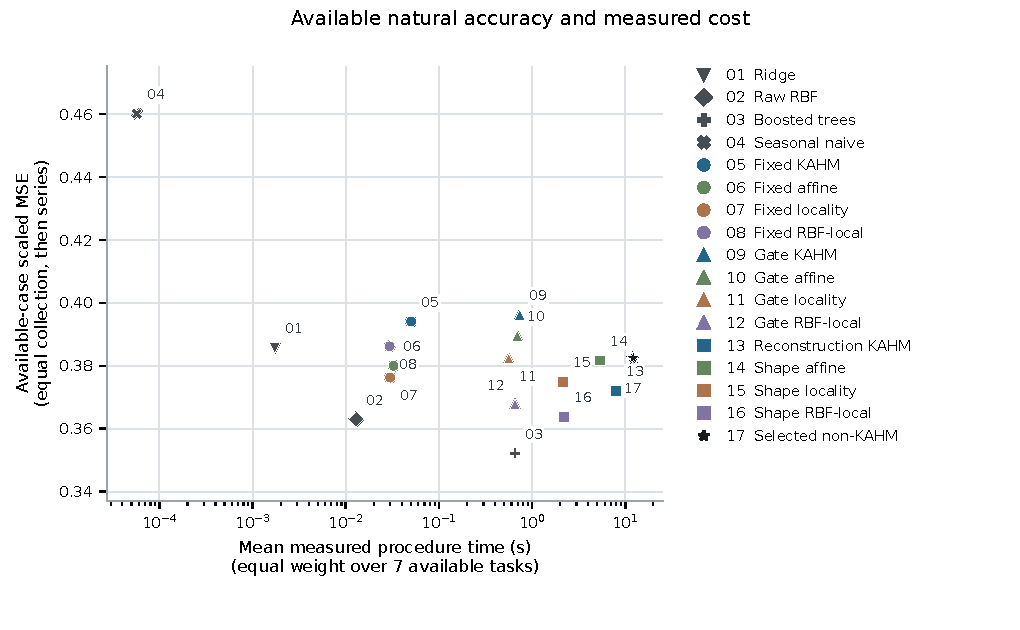
\includegraphics[width=\linewidth]{generated/direct_reconstruction/natural_available_accuracy_cost.pdf}
\caption{Available-case natural accuracy and implemented cost for all
17 procedures. Accuracy averages equally across three collections; time
averages equally across seven feasible task suites, with a logarithmic
horizontal scale. The missing rideshare collection is not replaced.
This descriptive plot does not establish population uncertainty or an
application-specific acceptable-cost threshold.}
\label{fig:direct-natural-cost}
\end{figure}
\FloatBarrier
